\documentclass{article}

% Page layout
\usepackage{geometry}
\geometry{
	a4paper,
}

% Fonts
\usepackage{fontspec}
\defaultfontfeatures{Mapping=tex-text,Scale=MatchLowercase}
\setmainfont{Linux Libertine O}

% Language
\usepackage{polyglossia}
\setdefaultlanguage{english}

% Graphics
\usepackage{graphicx}
\graphicspath{{./images/}}
\usepackage{dirtree}

% Links
\usepackage{url,hyperref}

% Headers and footers
\usepackage{fancyhdr}
\pagestyle{fancy}
\fancyhf{}
\setlength{\headheight}{25pt}
\lhead{
\includegraphics[scale=0.4]{inp-enseeiht}}
\rhead{
\includegraphics[scale=0.2]{irit}}
\lfoot{Install guide}
\rfoot{\bfseries \thepage}

% Code
\usepackage{verbatim}

\begin{document}

\sloppy

\vfill

\begin{center}
	{\Large Three-dimensional modelling and printing project}\\
	\bigskip
	{\Huge Install guide}\\
	\bigskip
	{\Large from January 23 to March 16, 2012}
\end{center}

\bigskip
\bigskip

\begin{center}
\large{
\textit{Vincent \textsc{Duvert} \\
Antoine \textsc{Lubineau} \\
Caroline \textsc{Naud} \\
James \textsc{Packer} \\
Florian \textsc{Ribon}} \\
\bigskip
INP-ENSEEIHT/IMA 
}
\end{center}

\vfill

\begin{figure}[!h]
\begin{center}
	
\includegraphics[scale=0.4]{inp-enseeiht}
\end{center}
\end{figure}

\bigskip

\begin{center}
\url{http://www.enseeiht.fr/fr/index.html} \\
2 Rue Charles Camichel \\
31 071 TOULOUSE
\end{center}

\vfill

\begin{figure}[!h]
\begin{center}
	
\includegraphics[scale=0.4]{irit}
\end{center}
\end{figure}

\begin{center}
\url{http://www.irit.fr}\\
Université Paul Sabatier \\
118 Route de Narbonne \\
F-31062 TOULOUSE CEDEX 9
\end{center}

\thispagestyle{empty}

\newpage

\tableofcontents

\newpage

\section{Global architecture of the application}

\begin{figure}[!h]
\begin{center}
	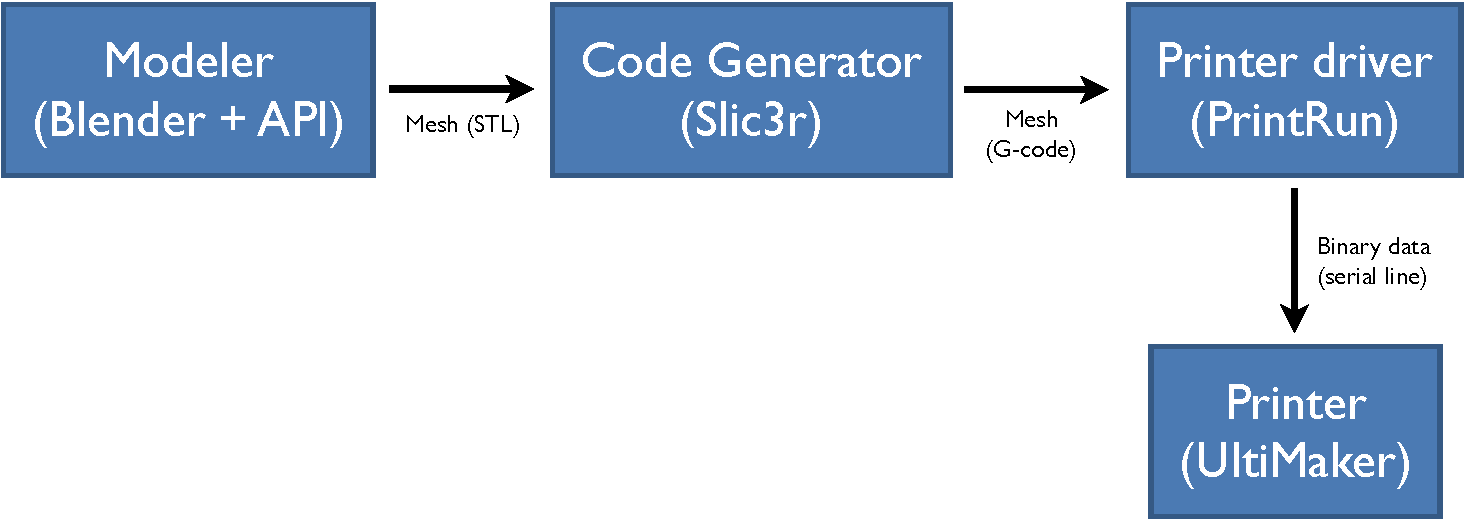
\includegraphics[width=\textwidth]{schema}
\end{center}
\end{figure}

Blender (and our API), Slic3r and PrintRun are user software whose will be needed to use the complete application. There is also a firmware integrated into the printer itself which may be updated (but this is not needed for our application).

\newpage

\section{Installing Blender}

	\paragraph{Description} Blender is a free, open-source and multi-platform 3D modelling software.

	\paragraph{Homepage} \url{http://www.blender.org/}

	\paragraph{Recommended version} \textbf{2.50 and later} because we use the Python 3 API, but scripts were only tested from versions 2.58 to 2.62 (latest available). From version 2.63, Blender will include BMesh, a complete rewrite of some parts of the modelling engine; the main change will be the support of n-sided polygons (instead of triangles and quads currently). This might break some of our functions, as the API will also change. Progress on integration of BMesh can be seen here: \url{https://bmeshblender.wordpress.com/}.

	\paragraph{Windows} Download the latest version on \url{http://www.blender.org/download/get-blender/}.

	\paragraph{Linux} Providing your distribution has a recent version of Blender, you should use your package manager. Else, you can download the 32~bits or 64~bits on \url{http://www.blender.org/download/get-blender/}.

	\paragraph{MaxOS X} Go to \url{http://www.blender.org/download/get-blender/}, download the version corresponding to your OS version, and follow the instructions in the provided \texttt{readme.html} file.

	\begin{figure}[h!]
		\centering
		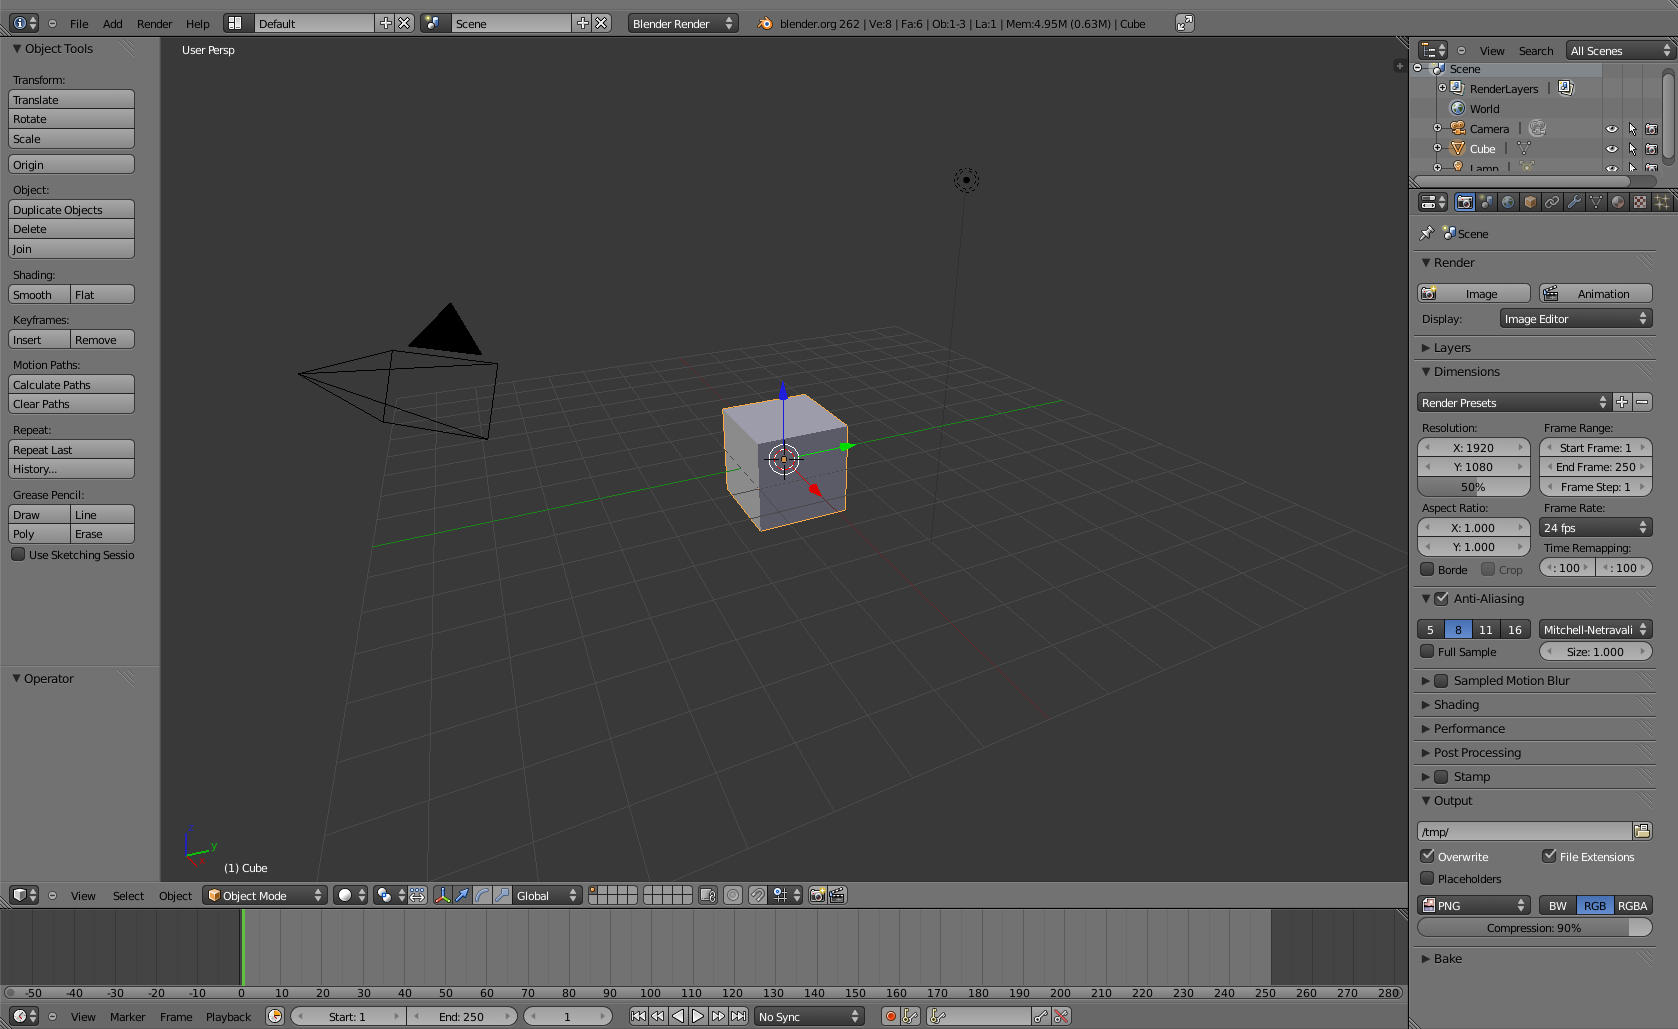
\includegraphics[width=\linewidth]{blender.png}
		\caption{Blender default interface}
	\end{figure}

\newpage

\section{Installing Slic3r}

	\paragraph{Description} Slic3r reads 3D models from STL files, and produces instructions for the printer as G-code (and M-code).

	\paragraph{Homepage} \url{http://slic3r.org/}

	\paragraph{Recommended version} \textbf{0.7.0 and later}, as it provides cooling support, better mesh slicing, binary compatibility with Ubuntu 11.10, etc.

	\paragraph{Windows} Go to \url{http://dl.slic3r.org/win/} and download \texttt{slic3r-mswin-x86-0-7-0.zip}. Extract the file, and you can launch \texttt{slic3r.exe} from the \texttt{Slic3r} folder.

	\paragraph{Linux} Go to \url{http://dl.slic3r.org/linux/} and download \texttt{slic3r-linux-x86-0-7-0.tar.gz}. To launch Slic3r:
		\begin{verbatim}
tar xf slic3r-linux-x86-0-7-0.tar.gz
cd Slic3r/bin
./slic3r
		\end{verbatim}
	If you have a 64-bit system, you will need to install the 32-bit support libraries (Debian/Ubuntu: \texttt{ia32-libs} and \texttt{ia32-libs-gtk} packages). You can install Slic3r by copying its folder into /opt and starting /opt/Slic3r/bin/slic3r (you will need to enable write permission for every user of the system to the contents of the /opt/Slic3r/lib/ folder).

	\paragraph{MaxOS X} Go to \url{http://dl.slic3r.org/mac/} and download \texttt{slic3r-osx-uni-0-7-0.dmg}. Open the disk image and drag the \emph{Slic3r} application to your Application folder. You can then start it by double-clicking on it.

	\begin{figure}[h!]
		\centering
		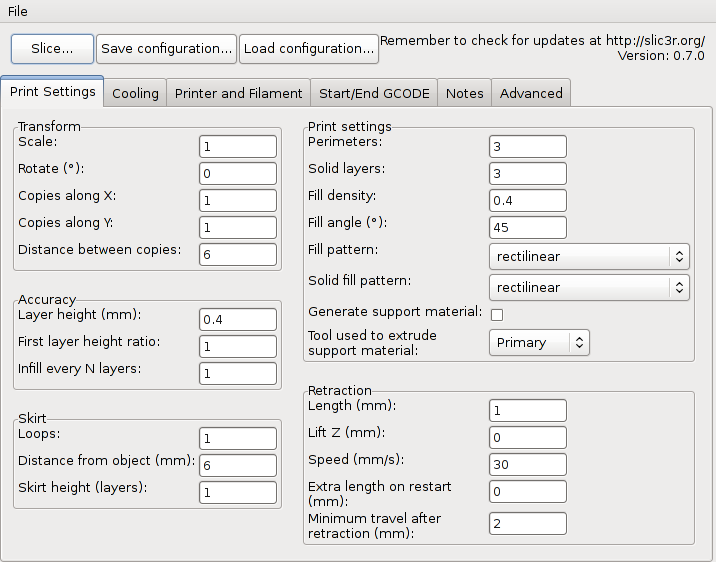
\includegraphics[width=0.6\linewidth]{slic3r.png}
		\caption{Slic3r interface}
	\end{figure}

	\paragraph{Alternatives} Skeinforge is also one the most popular slicing software. It has many more options than Slic3r, and is divided in modules. In some cases, the code makes less visible wires between parts of the objects. Yet it is more difficult to configure (many settings are not obvious), and it is quite slow (it relies on Psyco, a Python accelerator which is not more actively supported). It is available on \url{http://fabmetheus.crsndoo.com/}.

	\begin{figure}[h!]
		\centering
		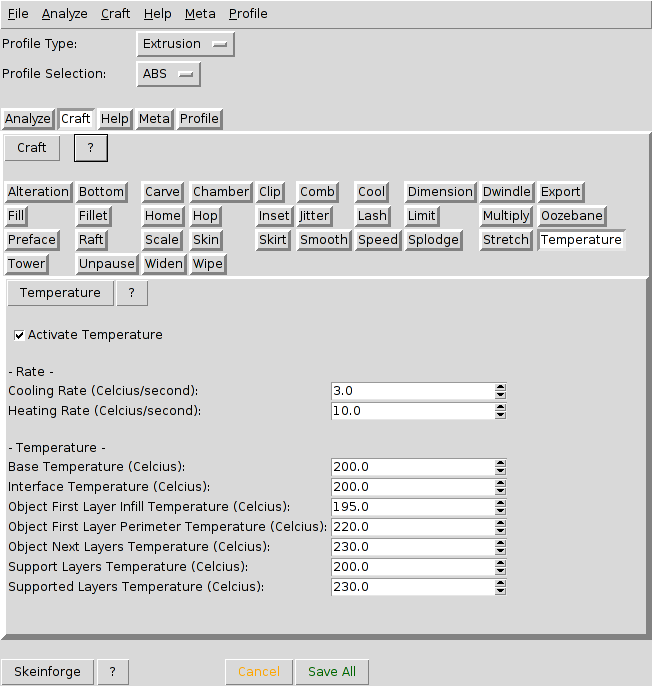
\includegraphics[width=0.6\linewidth]{skeinforge.png}
		\caption{Skeinforge interface}
	\end{figure}

\newpage

\section{Installing Blender plugin for printing and mesh preprocessing}

	\paragraph{Description} This plugin provides functions for checking that your meshes are fit to print.

	\paragraph{}
	You will need to locate the Blender data directory. Its location depends on
	the operating system. In the following description, \emph{<version>} is the
	Blender version you intend to use (for instance \texttt{2.62}). If you cannot find the mentioned folders, start Blender once and chose File~>~Save User Settings.

	\paragraph{Windows} The Blender data directory is \texttt{\emph{<your user profile>}\textbackslash{}Application Data\textbackslash{}Blender Foundation\textbackslash{}Blender\textbackslash{}\emph{<version>}\textbackslash{}}. The Application Data is a hidden folder, you can find it by opening the \emph{Run} panel (Start Menu>Run… or [Windows key]-R), and entering \texttt{\%APPDATA\%}. 

	\paragraph{Linux} The Blender data directory is \texttt{\~ {}/.blender/\emph{<version>}} (where \texttt{\~{}} is your user directory).
	
	\paragraph{Mac OS X} The Blender data directory is \texttt{\~{}/Library/Application Support/Blender/\emph{<version>}} (where \texttt{\~{}} is your user directory). If you cannot find the \texttt{Library} folder, press the Option (\emph{alt}) key and choose \emph{Library} in the \emph{Go} menu item.
	
	\paragraph{} Once you are in the Blender data directory, put the provided \texttt{scripts} folder in it. Then copy \texttt{startup.blend} in a \texttt{config} directory (it may or may not exist). You should have the following directory structure:\\

\dirtree{%
 .1 Blender data directory.
.2 config.
.3 startup.blend.
.2 scripts.
.3 modules.
.4 \_\_init\_\_.py.
.4 holes.py.
.4 manifold.py.
.4 planar\_faces.py.
.4 volume.py.
.3 startup.
.4 printing\_preprocessing.py.
}
	
	\paragraph{} If you are using Linux, make sure that the \texttt{zenity} utility is installed in order to see the progress dialogs (Under Debian/Ubuntu, you can install the \texttt{zenity} package)

	\begin{figure}[h!]
		\centering
		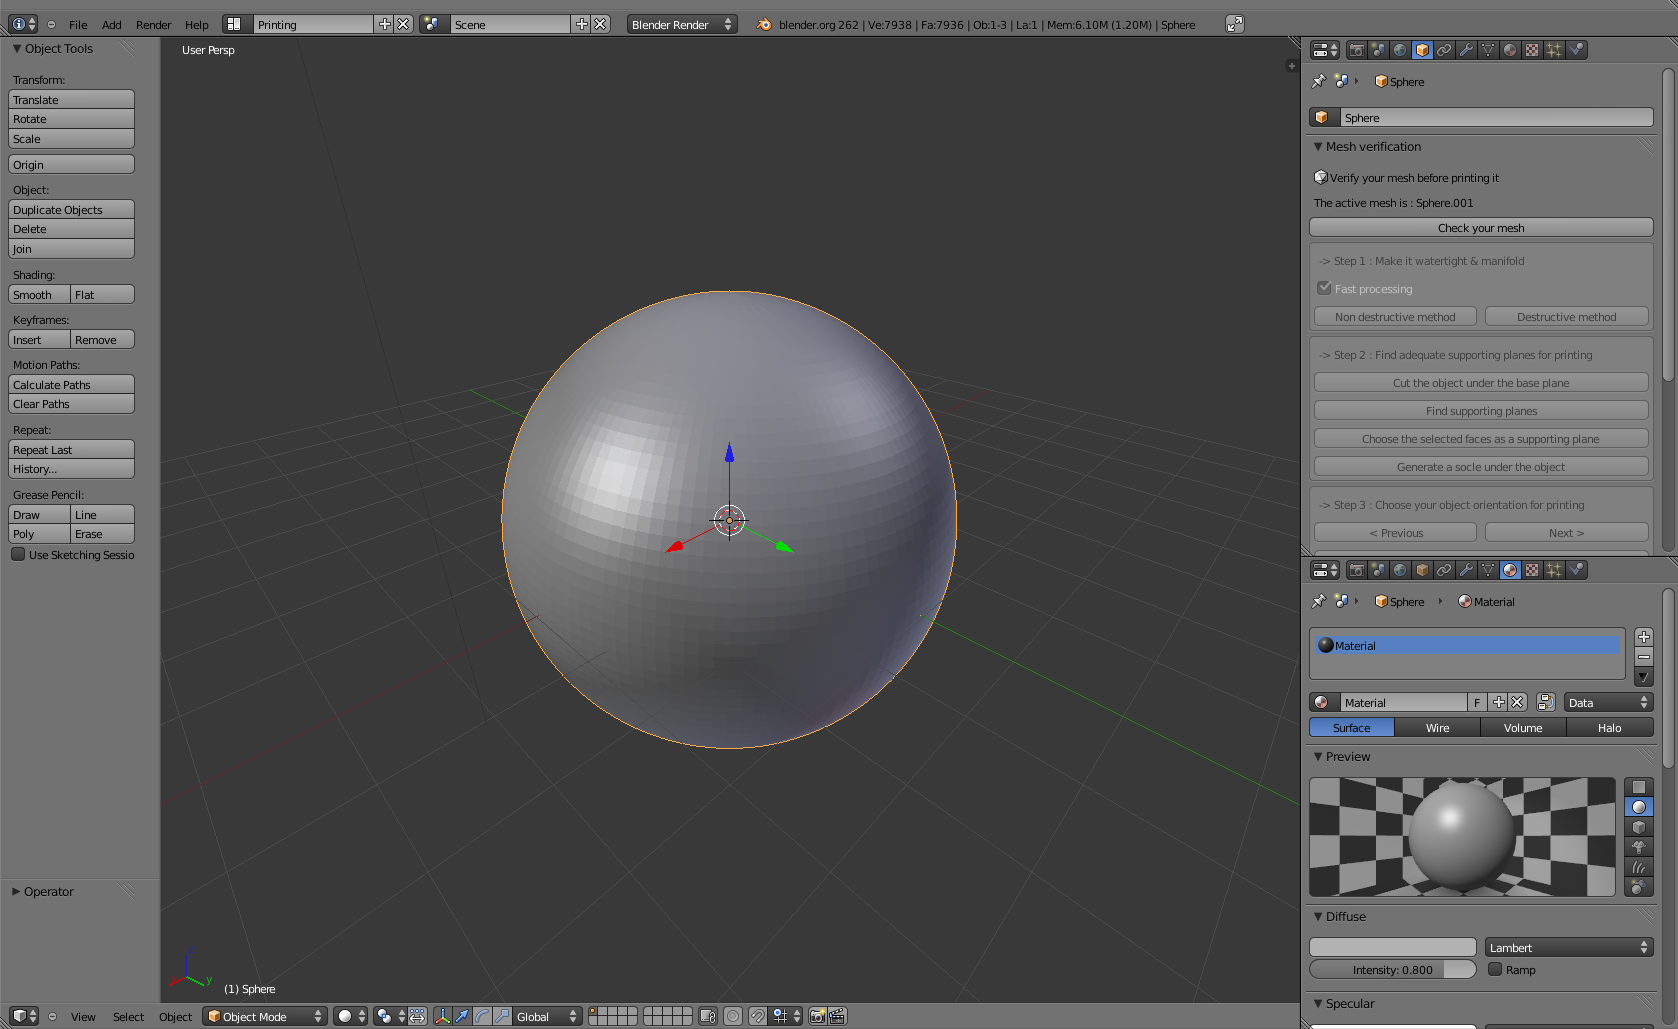
\includegraphics[width=\linewidth]{blender-plugin.png}
		\caption{Blender interface using the plugin}
	\end{figure}

	Once everything is installed, every time you start Blender, you should have a customized interface, with a new panel in the object editor, “Mesh verification”.

\newpage

\section{Installing Printrun}

	\paragraph{Description} Printrun is an interface for uploading G-code to the printer, and for manual piloting. One can also visualize the G-code in realtime while the object is printed.

	\paragraph{Home page} \url{https://github.com/kliment/Printrun}

	\paragraph{Installation} Instructions are available on \url{https://github.com/kliment/Printrun}. For Debian/Ubuntu, you can use the instructions provided on \url{http://reprap.org/wiki/Printrun}. Mac OS X users can download a pre-built executable at \url{http://koti.kapsi.fi/~kliment/printrun/pronterfacemac.zip}.

	\paragraph{Alternatives} ReplicatorG is also very used with 3D printers; it is available on \url{http://replicat.org/}. It comes bundled with Skeinforge, and it has a 3D preview.

	\begin{figure}[h!]
		\centering
		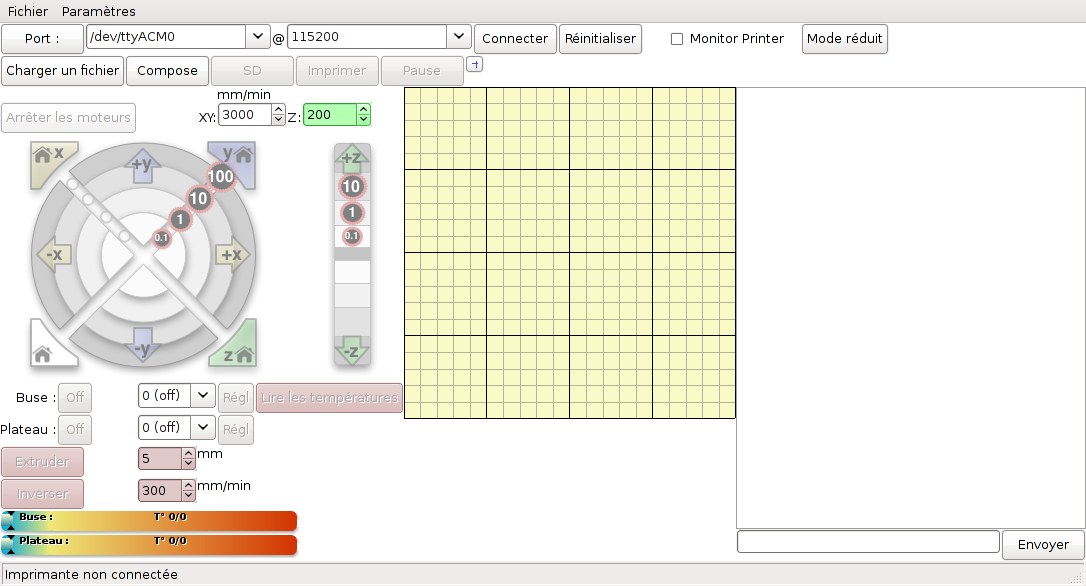
\includegraphics[width=0.7\linewidth]{printrun.png}
		\caption{Printrun main screen: printer controls on the left, object preview in the middle, and event logger on the right}
	\end{figure}

	\begin{figure}[h!]
		\centering
		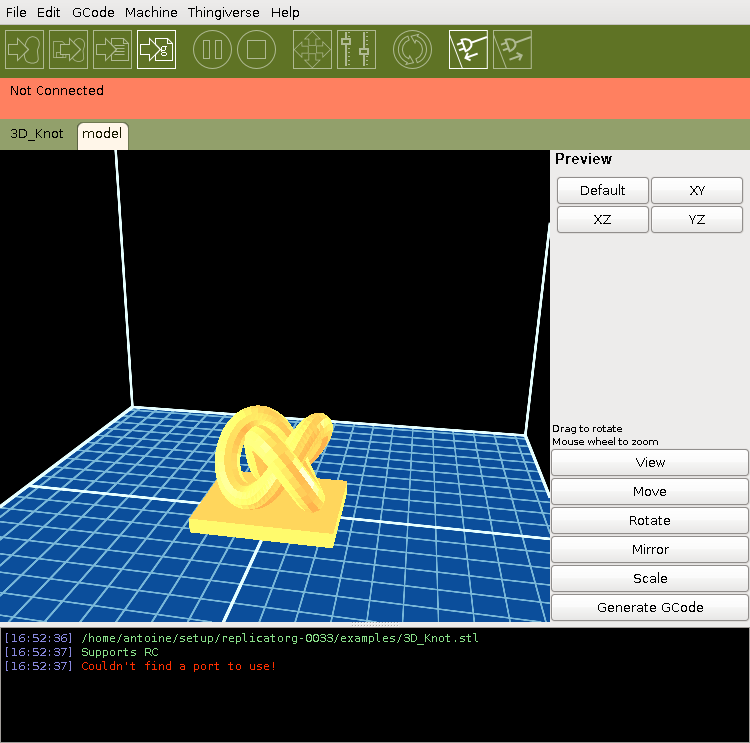
\includegraphics[width=0.5\linewidth]{replicatorg.png}
		\caption{ReplicatorG: 3D preview}
	\end{figure}
\end{document}
